\documentclass[11pt]{article}

\title{\textbf{ASSIGNMENT REPORT}}
\date{}
\usepackage{hyperref}
\hypersetup{
    colorlinks=true,
    linkcolor=black,
    filecolor=magenta,      
    urlcolor=black,
}
\usepackage{graphicx}\pagenumbering{roman}
\usepackage{geometry}
\geometry{margin=1.4in}
\pagenumbering{roman}
\begin{document}

\pagenumbering{gobble}% to remove numbering from title page
\begin{titlepage}
\centering
\vfill
\textbf{\Huge{Telecommunication Software Lab   %textbf makes the text bold and Huge make the font size large
\linebreak   %to introduce line break
\\ELP 718}}\\
\textcolor{red}{\rule{\textwidth}{3pt}}   %to introduce a red coloured bar
\vskip 2cm
\textbf{\Large{{\emph{Assignment No.7 Report}}}}\\
\vskip 0.5cm
\begin{figure}[h]
\centering

\includegraphics[scale=0.04]{iitdlogo}
\end{figure}
\section*{\center M.TECH}
\subsection*{\center BHARTI SCHOOL OF TELECOM TECHNOLOGY AND MANAGEMENT}
\bigskip
\bigskip
\bigskip
\bigskip
\bigskip
\bigskip
\begin{center}
\textbf{COURSE} : ELP-718-Telecom Software Laboratory\\
\textbf{YEAR} : 2016 \\
\textbf{SEMESTER} : I \\
\textbf{NAME} : Anant Khandelwal\\
\textbf{ENTRY NUMBER} :2016JTM2085 \\
\textbf{ASSIGNMENT NUMBER} :7\\
\textbf{ DATE} :\today
\end{center}
\end{titlepage}
\newpage

\begin{center} 
\renewcommand*\contentsname{Table Of Contents}
\tableofcontents
\newpage
\listoffigures
\newpage
\end{center}
\pagenumbering{arabic}
\newpage
\begin{center}
\section{Introduction}
\end{center}
\bigskip
\subsection{Python}
\begin{flushleft}
Python is a dynamic, interpreted (bytecode-compiled) language. There are no type declarations of variables, parameters, functions, or methods in source code. This makes the code short and flexible, and you lose the compile-time type checking of the source code. Python tracks the types of all values at runtime and flags code that does not make sense as it runs.\\\bigskip
An excellent way to see how Python code works is to run the Python interpreter and type code right into it. If you ever have a question like, "What happens if I add an int to a list?" Just typing it into the Python interpreter is a fast and likely the best way to see what happens\bigskip\\
\begin{figure}[h]
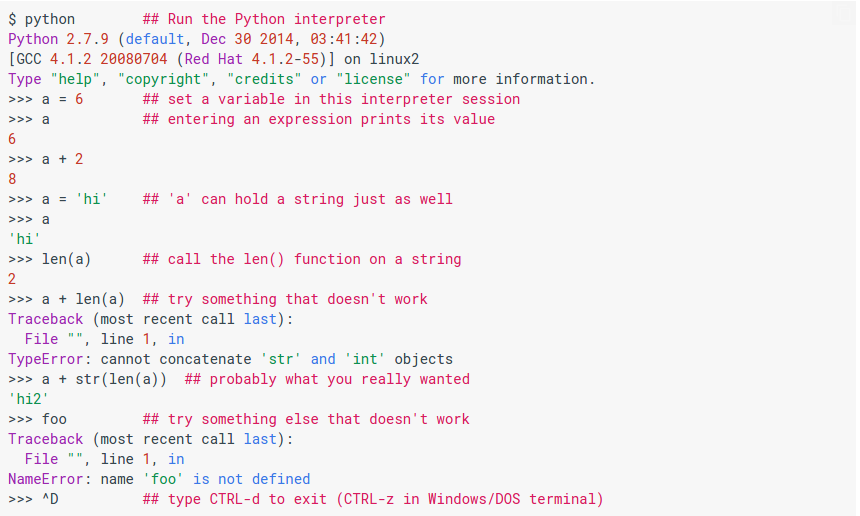
\includegraphics[scale=0.5]{python}
\centering
\caption{\textbf {Pyhton Interpreter}}
\end{figure}
Python source files use the ".py" extension and are called "modules."
\subsection{Github}
Git is a source code version control system, which a series of "commits" or snapshots of your code. You make the commits manually.\\
GitHub is a website (github.com) where you can publish your Git repositories for public download and possible collaboration.\\\bigskip
Specific steps to do this are:
\begin{itemize}
\item Install git and create a GitHub account 
\item Create a local git repository 
\item Add a new file to the repo
\item Add a file to the staging environment
\item Create a commit
\item Create a new branch
\item Create a new repository on GitHub
\item Push a branch to GitHub
\item Create a Pull Request (PR)
\item Merge a PR
\item Get changes on GitHub back to your computer
\item Bask in your git glory
\end{itemize}
\end{flushleft}
\newpage

\begin{center}
\section{Problem Statement­ - 1}
\end{center}
\bigskip
\begin{flushleft}
Write a Python program that can take a big string (with spaces) as input from the command line and count number of times a word occurs in the string and also print the top 3 words in terms of their frequency of count.
Also print the next permutation of each word appearing in the string.\\
\bigskip
Usage-
\subsection{Input Format}
\begin{itemize}
\item ./ps1.py  $<string>$       $=>$    
\end{itemize}
\subsection{Output Format}
\begin{itemize}
\item      $=>$ strings with frequency 
\end{itemize}
\end{flushleft}
\newpage

\begin{center}
\section{STRUCTURE CHART}
\end{center}
\bigskip
\begin{figure}[h]
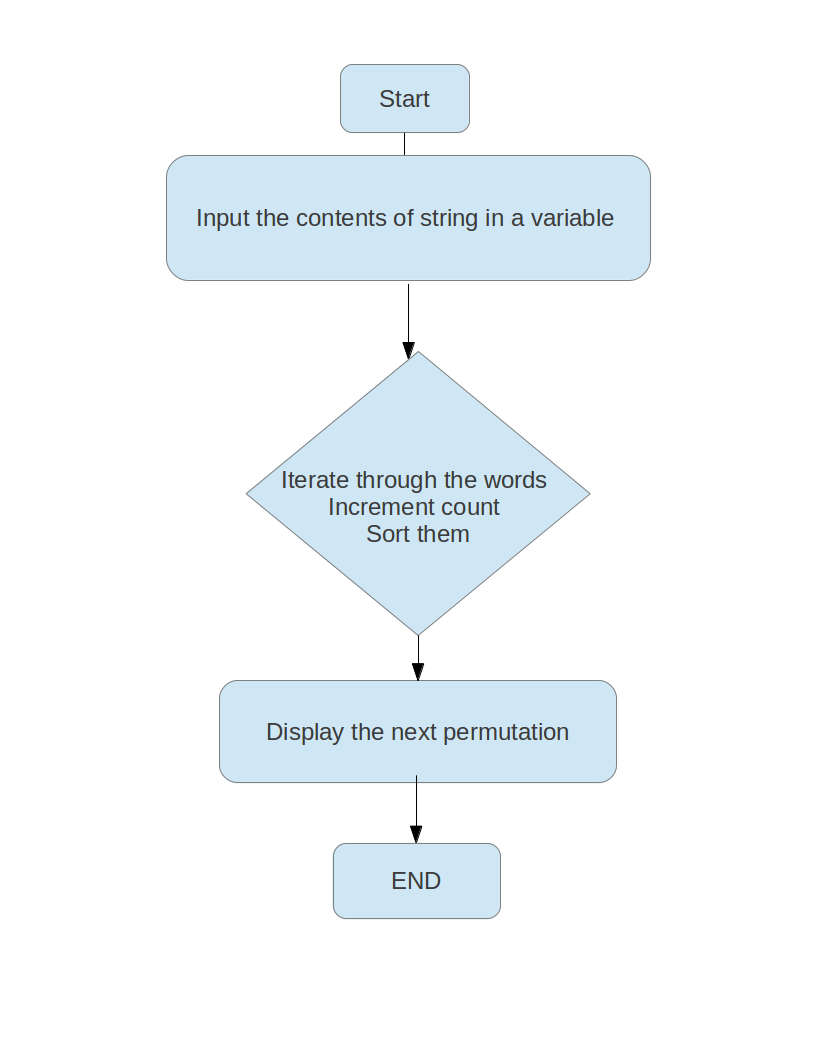
\includegraphics[scale=0.4]{structure}
\centering
\caption{Flow Diagram-1}
\end{figure}

\newpage
\begin{center}
\section{SCREENSHOTS}
\bigskip
\begin{figure}[h]
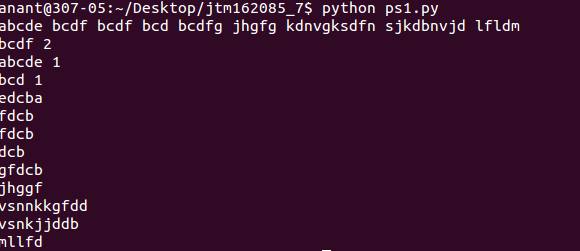
\includegraphics[scale=0.7]{p11}
\centering
\caption{Sample program Run - 1}
\end{figure}
\bigskip
\begin{figure}[h]
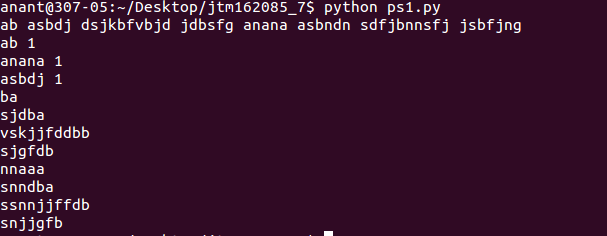
\includegraphics[scale=0.7]{p12}
\centering
\caption{Sample program Run - 1}
\end{figure}
\end{center}
\newpage
\begin{center}
\section{Problem Statement­ 2}
\end{center}
\bigskip
You are designing a Graphical user Interface (GUI) to depict the location of a mobile user in a square whose corner points are (1,1) (-1,1) (1,-1)(-1,-1). In real life, the user’s location would come from a database available with the MSC. For the moment, generate the user location using the random function generator function in Python to generate a number between [0,1). \\

Using following code generate points inside this 2D shape.(import random)\\

 (X,Y)=(random.random()*2- 1, random.random()*2-1)\\

 Here, each point in above shape has an equal chance of being generated.
Finally calculate number of points that lie inside unit radius circle in terms of percentage.\\
\newpage

\newpage

\begin{center}
\section{STRUCTURE CHART -PART 1}
\end{center}
\bigskip
\begin{figure}[h]
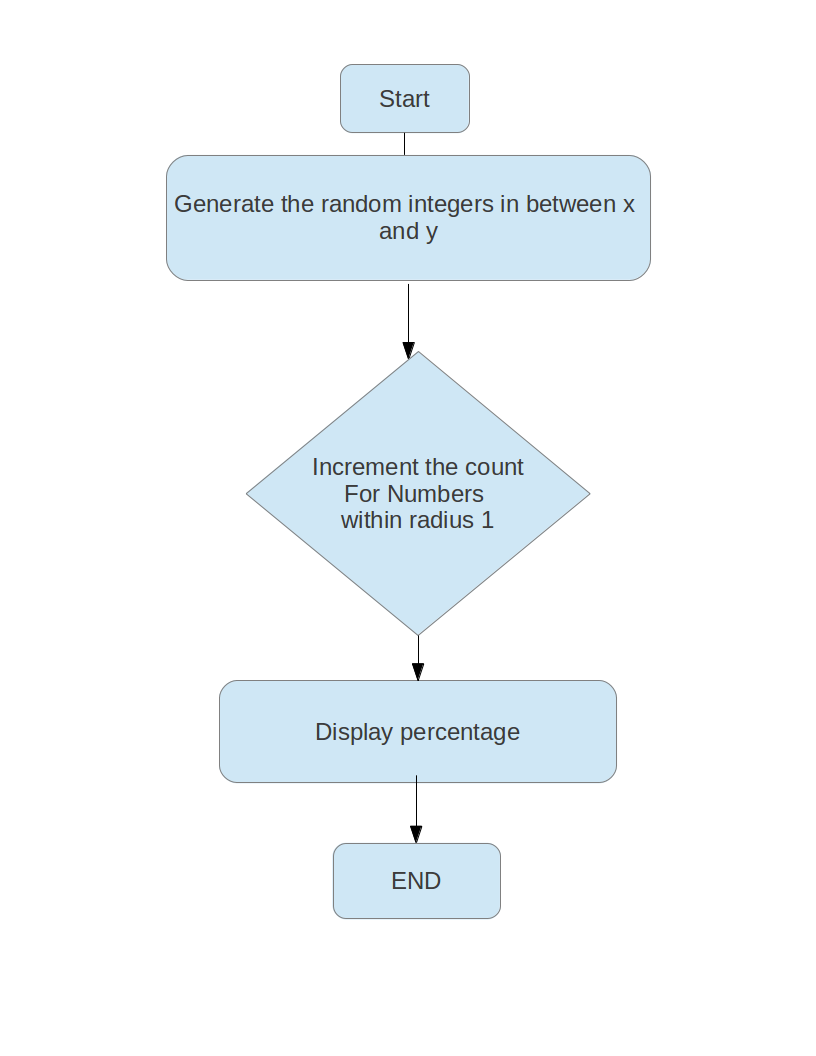
\includegraphics[scale=0.4]{structure1}
\centering
\caption{Flow Diagram-2}
\end{figure}
\newpage
\begin{center}
\section{Problem Statement­ 3}
\end{center}
\bigskip
You have to design an addressing code for a shipping company that works all around India. The address given by the customer is split into fields of 
Name, House No/colony/landmark\\
City\\
District\\
State/Union Territory\\
Let's suppose at the intake the employer enters all the above data into the computer, now the coding machine has to build two codes out of the data.\\

First is machine readable like barcodes, in the form 1’s and 0’s as:\\
IT Roorkee  $=$ 001\\
Roorkee $=$ 010\\
Uttarakhand $=$ 100\\
.
Second is human readable, build by combination of first three letters of a place.\\
For example :\\
Prof. Ram Mishra\\
D - 15, North Enclave\\
IIT Roorkee, Roorkee\\
Uttarakhand.\\

\begin{itemize}
\item Create a database with some default addresses.
\item The database should be editable(Add, delete, modify).
\item Also notify any discrepancy in data to the employee if the address is invalid or do not exist in the database.
\end{itemize}
\newpage
\begin{center}
\section{STRUCTURE CHART -PART 1}
\end{center}
\bigskip
\begin{figure}[h]
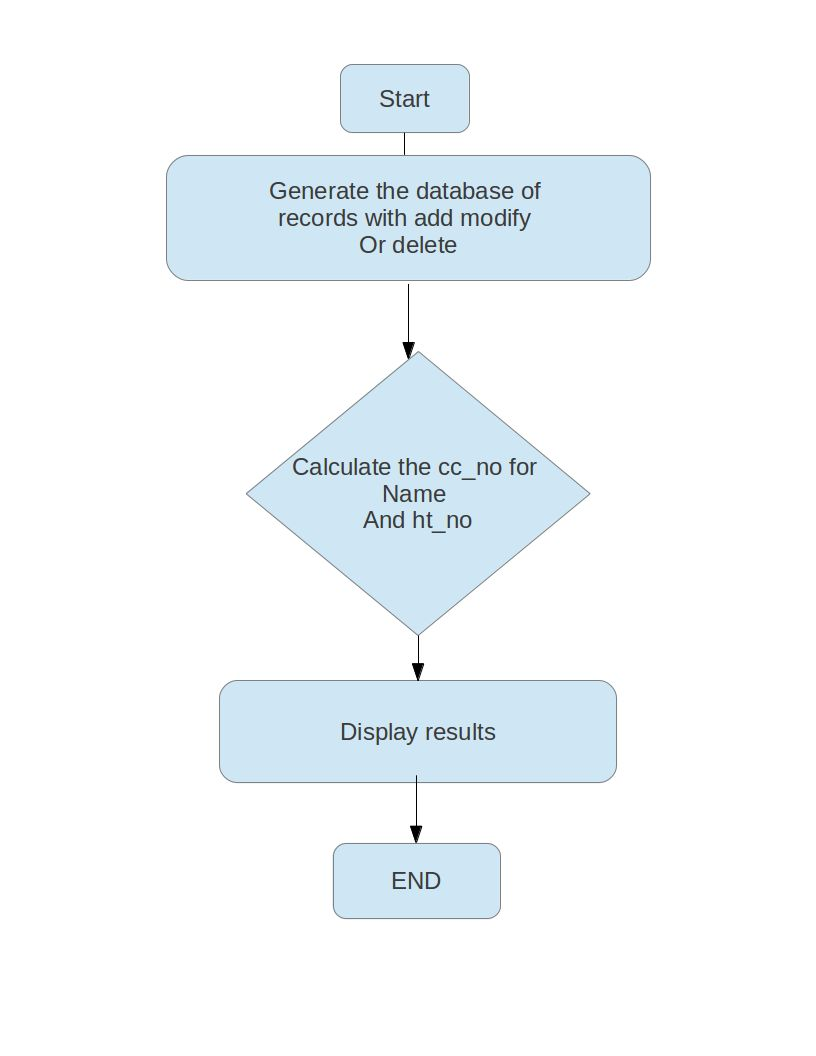
\includegraphics[scale=0.4]{structure2.jpg}
\centering
\caption{Flow Diagram-2}
\end{figure}
\newpage
\begin{center}
\section{SCREENSHOTS}
\bigskip

\begin{figure}[h]
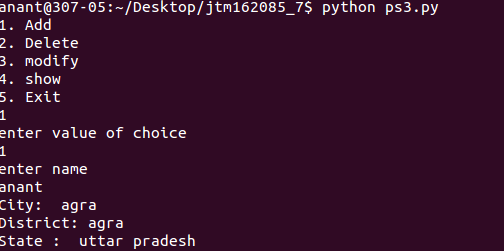
\includegraphics[scale=0.6]{PLAN1}
\centering
\caption{Sample program Run - 1}
\end{figure}
\end{center}
\begin{figure}[h]
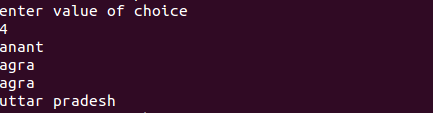
\includegraphics[scale=0.6]{PLAN2}
\centering
\caption{Sample program Run - 2}
\end{figure}
\begin{figure}[h]
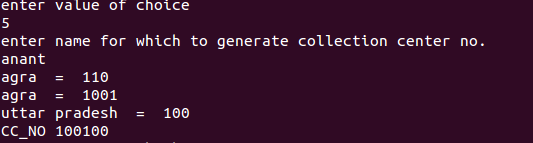
\includegraphics[scale=0.6]{PLAN3}
\centering
\caption{Sample program Run - 3}
\end{figure}
\newpage
\begin{figure}[h]
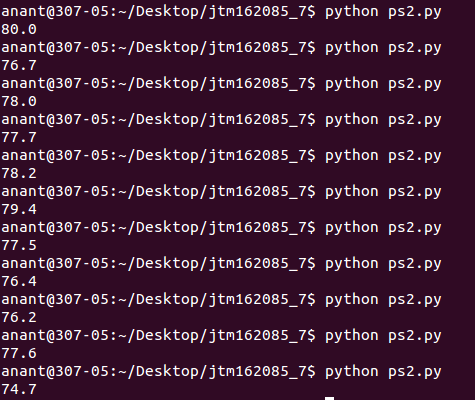
\includegraphics[scale=0.6]{p21}
\centering
\caption{Sample program Run - PART 2}
\end{figure}
\begin{figure}[h]
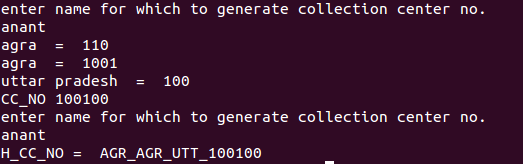
\includegraphics[scale=0.7]{p3}
\centering
\caption{Sample program Run - PART 3}
\end{figure}
\newpage
\newpage
\begin{center}
\begin{thebibliography}{9}
 
\bibitem{knuthwebsite} 
Hacker Rank: Python,
\\\texttt{\url {https://www.hackerrank.com/domains/python/py-introduction}}
\bibitem{} 
Tutorials point: Pyhton,
\\\texttt{\url {http://www.tutorialspoint.com/python/}}
\bibitem{} 
Google Developers: Python,
\\\texttt{\url {https://developers.google.com/edu/python/}}
\bibitem{} 
Udacity: Git and Github,
\\\texttt{\url {https://www.udacity.com/course/how-to-use-git-and-github--ud775}}
\end{thebibliography}
\end{center}
\addcontentsline{toc}{section}{REFERENCES}

\newpage
\begin{center}
\section*{EPILOGUE}
\end{center}
\bigskip
\begin{flushleft}
The assignment was very good in terms of learning the essence of logical thinking is required here.And the learning in that way that i learn about how to write the programs from the algorithm, taking the variables names.What caused me the grief is that while solving the problem which method i should use or i can say assumptions needs to be fulfilled or they can be removed so that it leads to a best program. 
\end{flushleft}
\addcontentsline{toc}{section}{EPILOGUE}
\end{document}